\documentclass[10pt,aspectratio=149]{beamer}

% All the boilerplate is in raslides.sty
% Note that this also pulls in a custom vogtwidebar.sty
\usepackage{raslides}

\author{Ji\v{r}\'i Lebl}

\institute[OSU]{%
Departemento pri Matematiko de Oklahoma {\^S}tata Universitato}

\title{BA: 1.3}

\date{}

\begin{document}

\begin{frame}
\titlepage
\end{frame}

\begin{frame}
The \emph{absolute value} is the size of $x \in \R$:
\[
\abs{x} \coloneqq
\begin{cases}
x & \text{if } x \geq 0, \\
-x & \text{if } x < 0 .
\end{cases}
\]

\pause

\begin{proposition}
\begin{enumerate}[(i)]
\item \label{prop:absbas:i} $\abs{x} \geq 0$, \quad moreover, $\abs{x}=0$ ~\iffif~ $x = 0$.
\item \pause \label{prop:absbas:ii} $\abs{-x} = \abs{x}$ \quad for all $x \in \R$.
\item \pause \label{prop:absbas:iii} $\abs{xy} = \abs{x}\abs{y}$ \quad for all $x,y \in \R$.
\item \pause \label{prop:absbas:iv} $\abs{x}^2 = x^2$ \quad for all $x \in \R$.
\item \pause \label{prop:absbas:v} $\abs{x} \leq y$ \wiffif $-y \leq x \leq y$.
\item \pause \label{prop:absbas:vi} $-\abs{x} \leq x \leq \abs{x}$ \quad for all $x \in \R$.
\end{enumerate}
\end{proposition}

\pause

\textbf{Proof:}
\eqref{prop:absbas:i}:

Case $x \geq 0$:
\quad
\pause
$\abs{x} = x \geq 0$
\quad
\pause
also $\abs{x} = x = 0$ ~\iffif~ $x=0$.

\pause
Case $x < 0$:
\quad
$\abs{x} = -x > 0$ \quad \pause and $\abs{x} \not= 0$.

\end{frame}

\begin{frame}

\eqref{prop:absbas:ii} ``$\abs{-x} = \abs{x}$ for all $x \in \R$'':

\pause
Case $x > 0$: \pause \quad $-x < 0$ \pause \wthus $\abs{-x} = -(-x) = x = \abs{x}$.

\pause
Cases $x < 0$ and $x=0$ similar.

\medskip
\pause

\eqref{prop:absbas:iii} ``$\abs{xy} = \abs{x}\abs{y}$ for all $x,y \in \R$'':

\pause
Case $x=0$ or $y=0$: immediate.

\pause
Case $x > 0$ \& $y > 0$: \pause
\quad $xy > 0$ \pause \wthus
$\abs{xy} = xy \pause = \abs{x} \abs{y}$.

\pause
Case $x < 0$ \& $y < 0$: \pause
\quad $xy = (-x)(-y) > 0$ \pause
\wthus
$\abs{xy} = xy = (-x)(-y) = \abs{x} \abs{y}$.

\pause
Case $x > 0$ \& $y < 0$: \pause
\quad
$xy < 0$
\pause
\wthus
$\abs{xy} = -(xy) = x(-y) = \abs{x}\abs{y}$.

\pause
Case $x < 0$ \& $y > 0$ is similar.

\medskip
\pause

\eqref{prop:absbas:iv} ``$\abs{x}^2 = x^2$ for all $x \in \R$'':

\pause
Case $x \geq 0$: immediate.

\pause
Case $x < 0$: \pause \quad $\abs{x}^2 = {(-x)}^2 = x^2$.

\end{frame}

\begin{frame}

\eqref{prop:absbas:v} ``$\abs{x} \leq y$ \wiffif $-y \leq x \leq y$'':

\medskip
\pause

Suppose $\abs{x} \leq y$.  As $\sabs{x} \geq 0$ \wthus $y \geq 0$.

\pause
Case $x \geq 0$:
\pause \quad $x \leq y$ \pause \quad , \quad $y \geq 0$ \pause \wthus $-y
\leq 0 \leq x$ \pause \wthus $-y \leq x \leq y$.

\pause
Case $x < 0$: \pause \quad $-x = \abs{x} \leq y$ \pause \wthus
$x \geq -y$ \pause \quad , \quad $y \geq 0 \pause > x$ \wthus
$-y \leq x \leq y$.

\medskip
\pause

Now suppose
$-y \leq x \leq y$.

\pause
Case $x \geq 0$: \pause \quad $y \geq x \pause = \abs{x}$.

\pause
Case $x < 0$: \pause \quad $-y \leq x$ \pause \wthus
$y \geq -x \pause = \abs{x}$.

\medskip
\pause

\eqref{prop:absbas:vi} ``$-\abs{x} \leq x \leq \abs{x}$ for all $x \in \R$'':

\pause
\eqref{prop:absbas:v} with $y = \abs{x}$.
\qed
\end{frame}

\begin{frame}

\begin{proposition}[Triangle Inequality]
$\sabs{x+y} \leq \sabs{x}+\sabs{y}$
for all $x, y \in \R$.
\end{proposition}

\pause

\textbf{Proof:}
By the previous proposition \quad
$- \sabs{x} \leq x \leq \sabs{x}$ and
$- \sabs{y} \leq y \leq \sabs{y}$.

\pause
Add the two: \quad $- \bigl(\sabs{x}+\sabs{y}\bigr) \leq x+y \leq \sabs{x}+ \sabs{y}$.

\pause
By the proposition again \quad
$\sabs{x+y} \leq \sabs{x}+\sabs{y}$.
\qed

\medskip
\pause

E.g.,

\pause
$3 = \abs{1+2} \leq \abs{1}+\abs{2} = 1+2$

\pause
$1 = \abs{1-2} = \abs{1+(-2)} \leq \abs{1}+\abs{-2} = 1+2=3$

\end{frame}

\begin{frame}

\begin{corollary}
Let $x,y \in \R$.
\begin{enumerate}[(i)]
\item \emph{(reverse triangle inequality)}
~
$\bigl\lvert (\abs{x}-\abs{y}) \bigr\rvert \leq \abs{x-y}$.
\item \pause$\abs{x-y} \leq \abs{x}+\abs{y}$.
\end{enumerate}
\end{corollary}
\pause

\textbf{Proof:}
(i) Plug $x=a-b$ and $y=b$ into the standard triangle inequality:

$\abs{a} = \abs{a-b+b} \leq \abs{a-b} + \abs{b}$
\pause
\wthus
$\abs{a}-\abs{b} \leq \abs{a-b}$

\pause
Switch roles of $a$ and $b$:

$\abs{b}-\abs{a} \leq \abs{b-a} = \abs{a-b}$

\pause
(i) follows.

\medskip
\pause

(ii): Replace $y$ with $-y$ in standard triangle inequality.
\qed

\medskip
\pause

E.g.,

$2=3-1=\abs{3}-\abs{1} \leq \abs{3-1} = 2$

\pause
$2=3-1=\abs{-3}-\abs{1} \leq \abs{-3-1} = 4$

\end{frame}

\begin{frame}

\begin{corollary}
Let $x_1, x_2, \ldots, x_n \in \R$.  Then
\begin{equation*}
\abs{x_1 + x_2 + \cdots + x_n} \leq 
\abs{x_1} + \abs{x_2} + \cdots + \abs{x_n} .
\end{equation*}
\end{corollary}
\pause

\textbf{Proof:}
Induction!

\medskip
\pause

Trivial if $n=1$.

\medskip
\pause

Suppose conclusion holds for $n$ numbers.

\pause
Consider $n+1$ numbers $x_1,x_2,\ldots,x_{n+1}$.

\pause
\medskip

$\displaystyle
\sabs{x_1 + x_2 + \cdots + x_n + x_{n+1}} \leq 
\sabs{x_1 + x_2 + \cdots + x_n} + \sabs{x_{n+1}}$

\medskip
\pause
$\displaystyle
\hspace{1.53in}\leq 
\sabs{x_1} + \sabs{x_2} + \cdots + \sabs{x_n} + \sabs{x_{n+1}}
$
\qed
\end{frame}

\begin{frame}

\textbf{Example:}
Find a number $M$ such that $\sabs{x^2-9x+1} \leq M$ for all $-1 \leq x \leq
5$.

\pause
\medskip


$
\sabs{x^2-9x+1} \leq \sabs{x^2}+\sabs{9x}+\sabs{1}
\pause
=
\sabs{x}^2+9\sabs{x}+1 .
$

\medskip
\pause

$\sabs{x}^2+9\sabs{x}+1$ is largest when $\abs{x}$ is largest (why?).

\medskip
\pause

$\abs{x}$ is largest when $\abs{x}=5$.

\medskip
\pause

So a possible $M = 5^2+9(5)+1 = 71$.

\medskip
\pause

Other $M$ work.  E.g., $M=100$ works.

\pause
A little calculus shows $M=\nicefrac{77}{4}=19.25$ would also work (least such $M$).

\medskip
\pause

We didn't ask for the best $M$, any $M$ that works will do.

\medskip
\pause

That sort of point comes up often in analysis.

\end{frame}

\begin{frame}

\begin{definition}
$f \colon D \to \R$ is
\emph{bounded}
if $\exists$ $M$
such that $\abs{f(x)} \leq M$ for all $x \in D$.
\end{definition}

\pause

We proved $x^2-9x+1$ is bounded when the domain is $D = \{ x : -1 \leq x \leq 5 \}$.


\medskip
\pause

If we make $D=\R$, then $x^2-9x+1$ is not bounded.

\medskip
\pause

We write: \quad 
$\displaystyle \sup_{x \in D} f(x) \coloneqq \sup\, f(D)$
\quad
$\displaystyle \inf_{x \in D} f(x) \coloneqq \inf\, f(D)$

\medskip
\pause

We also write: \quad 
$\displaystyle
\sup_{-1 \leq x \leq 5} ( x^2 -9x+1 ) = 11$
\quad
$\displaystyle\inf_{-1 \leq x \leq 5} ( x^2 -9x+1 ) = \nicefrac{-77}{4}$ .

\medskip
\pause

\begin{center}
\scalebox{0.85}{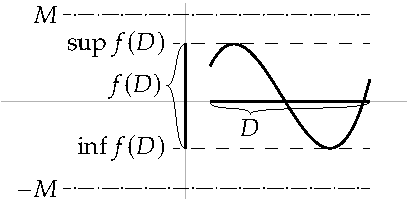
\includegraphics{../figures/boundedfunc}}
\end{center}

\end{frame}

\begin{frame}
\begin{proposition}
If $f \colon D \to \R$, $g \colon D \to \R$ ($D\not= \emptyset$) are
bounded and
$f(x) \leq g(x)$ for all $x \in D$, then
\[
\sup_{x \in D} f(x) \leq \sup_{x \in D} g(x)
\qquad \text{and} \qquad
\inf_{x \in D} f(x) \leq \inf_{x \in D} g(x) .
\]
\end{proposition}

\pause

\textbf{Caution:}
The $x$ on the LHS is different than the $x$ on the RHS. \pause Perhaps think
\[
\sup_{x \in D} f(x) \leq \sup_{y \in D} g(y) .
\]

\pause
\textbf{Proof:} We prove the sup, leave the inf as exercise.

\pause
Suppose $b$ is an upper bound for $g(D)$.

\pause
\thus \quad
$f(x) \leq g(x) \leq b$ for all $x \in D$
\pause
\wthus
$b$ is an upper bound for $f(D)$.

\pause
Taking the LUB of $g(D)$ gets $\displaystyle
f(x) \leq \sup_{y \in D} g(y)$ for any $x \in D$.

\pause
So the LUB of $g(D)$ is an upper bound for $f(D)$.

\pause
\thus \quad
$\displaystyle \sup_{x \in D} f(x) \leq \sup_{y \in D} g(y)$
\qed

\end{frame}

\begin{frame}

\textbf{Caution:}
$f(x) \leq g(x)$ for all $x \in D$ does \textbf{NOT} imply
$\displaystyle
\sup_{x \in D} f(x) \leq \inf_{y \in D} g(y)$.

\medskip
\pause

For this you need every value of $g(y)$ to be a bound for $f$:

\pause
\medskip

That is,
$f(x) \leq g(y)$ for all $x,y \in D$ does imply
$\displaystyle
\sup_{x \in D} f(x) \leq \inf_{y \in D} g(y)$.

\pause
\medskip

Proof is an exercise.

\end{frame}

\begin{frame}

\textbf{Exercise:}
Let $D$ be nonempty and
$f \colon D \to \R$, $g \colon D \to \R$ be bounded.
\begin{enumerate}[a)]
\item
\pause
Show 
\[
\sup_{x\in D} \bigl(f(x) + g(x) \bigr) \leq
\sup_{x\in D} f(x)
+
\sup_{x\in D} g(x)
\]
\pause
and
\[
\inf_{x\in D} \bigl(f(x) + g(x) \bigr) \geq
\inf_{x\in D} f(x)
+
\inf_{x\in D} g(x) .
\]
\item
\pause
Find examples where we obtain strict inequalities.
\end{enumerate}

\end{frame}

\end{document}
